% Created 2022-06-29 Wed 16:43
% Intended LaTeX compiler: pdflatex
\documentclass[presentation,aspectratio=169]{beamer}
\usepackage[utf8]{inputenc}
\usepackage[T1]{fontenc}
\usepackage{graphicx}
\usepackage{grffile}
\usepackage{longtable}
\usepackage{wrapfig}
\usepackage{rotating}
\usepackage[normalem]{ulem}
\usepackage{amsmath}
\usepackage{textcomp}
\usepackage{amssymb}
\usepackage{capt-of}
\usepackage{hyperref}
\usepackage{khpreamble}
\usepackage{amssymb}
\usepackage{mathtools}
\usepgfplotslibrary{groupplots}
\DeclareMathOperator{\shift}{q}
\DeclareMathOperator{\diff}{p}
\usetheme{default}
\author{Kjartan Halvorsen}
\date{2022-06-29}
\title{Sampling and aliasing}
\hypersetup{
 pdfauthor={Kjartan Halvorsen},
 pdftitle={Sampling and aliasing},
 pdfkeywords={},
 pdfsubject={},
 pdfcreator={Emacs 26.3 (Org mode 9.4.6)}, 
 pdflang={English}}
\begin{document}

\maketitle

\section{Intro}
\label{sec:orga4dcdd2}

\begin{frame}[label={sec:org129a739}]{Computer-controlled system}
\begin{center}
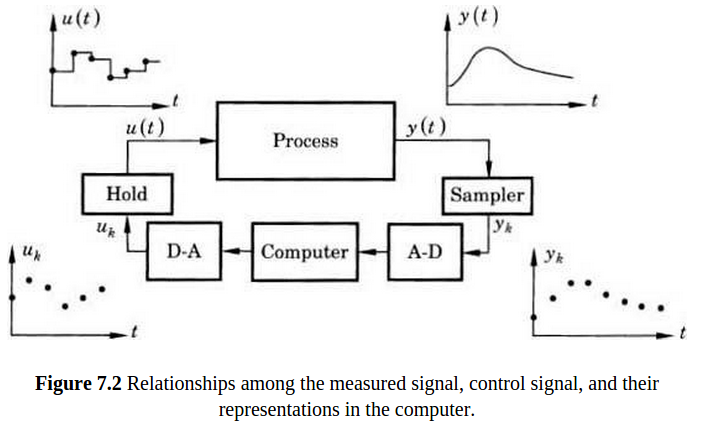
\includegraphics[width=0.7\linewidth]{../../figures/fig7-2.png}
\end{center}
{\footnotesize Source: Åström \& Wittenmark}
\end{frame}


\section{The sampling theorem}
\label{sec:org1a7350f}
\begin{frame}[label={sec:org669fc95}]{Challenges with computerized control - aliasing}
\begin{columns}
\begin{column}{0.6\columnwidth}
\begin{center}
  \begin{tikzpicture}
    \node {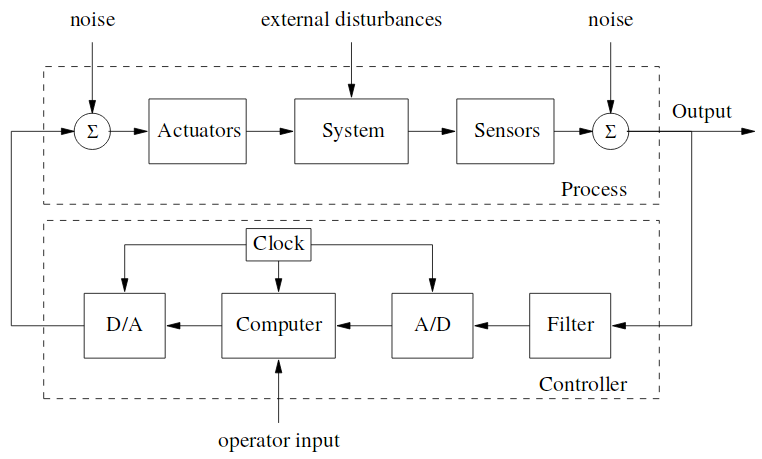
\includegraphics[width=0.99\linewidth]{../../figures/comp-contr-sys.png}};
    \node[pin=145:{60Hz mains hum}] at (2.7,2.4) {};
    \node[pin=-60:{90Hz sampling freq}] at (0.5,-1.4) {};
  \end{tikzpicture}
\end{center}
\end{column}
\begin{column}{0.4\columnwidth}
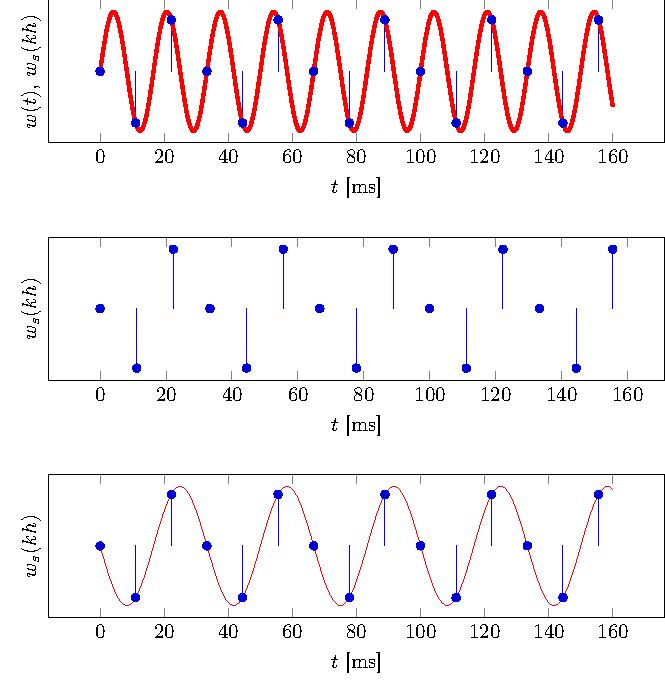
\includegraphics[width=0.99\linewidth]{../../figures/aliasing-example-60Hz}
\end{column}
\end{columns}
\end{frame}

\begin{frame}[label={sec:orgb4c6c49}]{Spatial aliasing}
\begin{center}
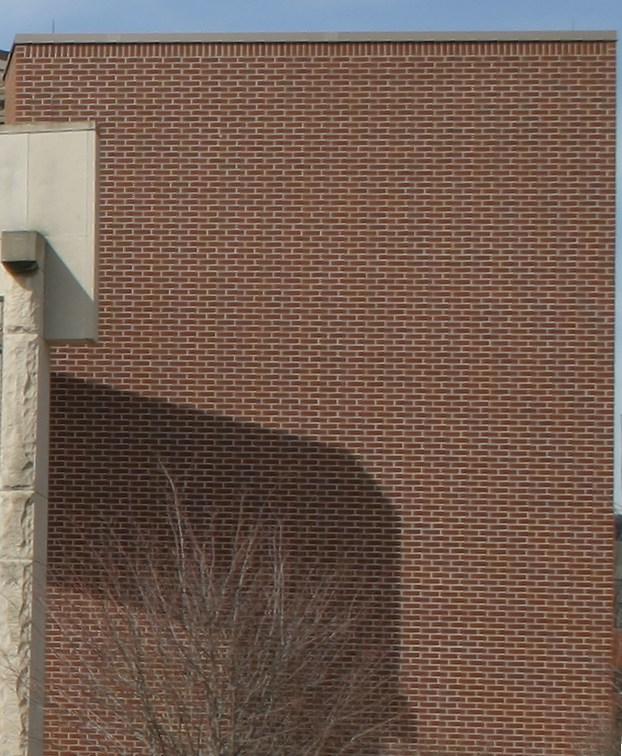
\includegraphics[width=0.45\linewidth]{../../figures/Moire_pattern_of_bricks.png}
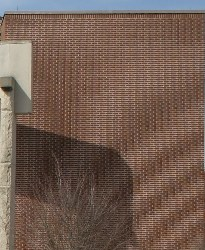
\includegraphics[width=0.45\linewidth]{../../figures/Moire_pattern_of_bricks_small.png}
\end{center}
\end{frame}

\begin{frame}[label={sec:orgf31eac7}]{The sampling theorem}
Shannon and Nyquist:

A continuous-time signal with Fourier transform that is zero outside the interval \((-\omega_0, \omega_0)\)  can be completely reconstructed from equidistant samples of the signal, as long as the sampling frequency is at least \(2\omega_0\). 

\begin{center}
  \begin{tikzpicture}[scale=1.2]
    \draw[->] (-3,0) -- (3,0) node[below] {$\omega$};
    \draw[->] (0,0) -- (0,1.5);
    \draw[red, thick] (0,1) to (1,0);
    \draw[red, thick] (0,1) to (-1,0);
    \node at (1,-0.3) {$\omega_0$};
    \node at (-1,-0.3) {$-\omega_0$};
    \node at (0,-0.3) {$0$};
    \node[coordinate, pin=-90:{$2\omega_0$}] at (2,0) {};

  \end{tikzpicture}
\end{center}
\end{frame}

\begin{frame}[label={sec:org74deb48}]{The impulse modulation model}
The \alert{impulse train}, a.k.a the \alert{Dirac comb}:
\begin{center}
\(m(t) = \sum_{k=-\infty}^{\infty} \delta(t-kh)\)\hspace*{10mm}
 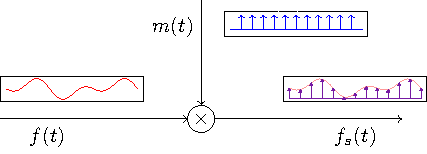
\includegraphics[width=0.6\linewidth]{../../figures/modulation-model-blocks}
\end{center}

\pause
\[f_s(t) = f(t)m(t) = f(t) \sum_{k=-\infty}^{\infty} \delta(t-kh) \quad\xleftrightarrow{\mathcal{F}}\quad F_s(\omega) = F(\omega) \ast M(\omega)\]

\pause

\footnotesize

\begin{block}{Resources}
\href{https://youtu.be/SxNVcCVj-3c}{Dr. Trefor Bazett on the Dirac delta function, }
\href{https://youtu.be/TIcfY19dk0c}{Prof Iain Collings explains convolution with the delta, }
\href{https://youtu.be/nHguB7MvCfI}{Steven Fenton on the dirac comb and sampling}
\end{block}
\end{frame}

\begin{frame}[label={sec:org0261dd9}]{Fourier transform of the sampled signal}
The Fourier transform of \(f_s\) and the Fourier transform of \(f\) are related as
\[ F_s(\omega) = \frac{1}{h} \sum_n F(\omega + n\omega_s). \]

Because the Fourier transform of the sampled signal equals the Fourier transform of the continuous-time signal repeated at every multiple of the sampling frequency and added, we get \emph{frequency-folding} or \emph{aliasing}.

\begin{center}
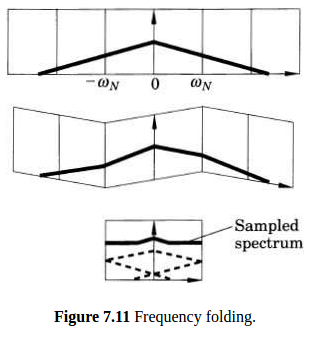
\includegraphics[width=0.28\linewidth]{../../figures/frequency-folding.png}
\end{center}
\end{frame}

\section{Exercises using line spectra}
\label{sec:org432a0f9}
\begin{frame}[label={sec:org9586866}]{Fourier transform of a complex exponential}
\small 
The function \(x(t) = \mathrm{e}^{i\omega_1 t}\) 
\begin{center}
  \begin{tikzpicture}[scale=1.4]
    \draw[->] (-1.2, 0) -- (1.2,0) node[below] {Re};
    \draw[->] (0, -1.2) -- (0,1.2) node[left] {Im};
    \draw[domain=0:360, samples=361, dashed] plot ({cos(\x)}, {sin(\x)});
    \node[circle, fill, inner sep=2pt, red] (pnt) at (0.868, 0.5) {};
    \draw[dashed, blue] (0,0) to (0.868, 0.5);
    \draw[domain=0:30, samples=20, ->] plot ({0.6*cos(\x)}, {0.6*sin(\x)});
    \node at (0.7, 0.2) {$\omega_1 t$};
    \node[pin=-135:{1}, coordinate] at (1, 0) {};
    \node[right of=pnt, node distance=3mm, anchor=west] {$x(t) = \mathrm{e}^{i\omega_1 t} = \cos(\omega_1 t) + i\sin(\omega_1 t)$};
  \end{tikzpicture}
\end{center}

\pause
has Fourier transform 
   \[X(i\omega) = \int_{-\infty}^{\infty} x(t) \mathrm{e}^{-i\omega t}dt = \int_{-\infty}^{\infty} \mathrm{e}^{i(\omega_1 - \omega) t}dt = 2\pi \delta(\omega_1 - \omega)\] 

\footnotesize
\begin{block}{Resources}
\href{https://youtu.be/TLWE388JWGs}{Prof Iain Collings on Complex numbers and real signals}
\end{block}
\end{frame}

\begin{frame}[label={sec:org1c1caa6}]{Fourier transform of a sinusoid}
A sinusoidal signal \(y(t) = \sin(\omega_1 t)\) has all its power concentrated at one single frequency, \(\omega=\unit{\omega_1}{rad\per\second}\). 
\begin{center}
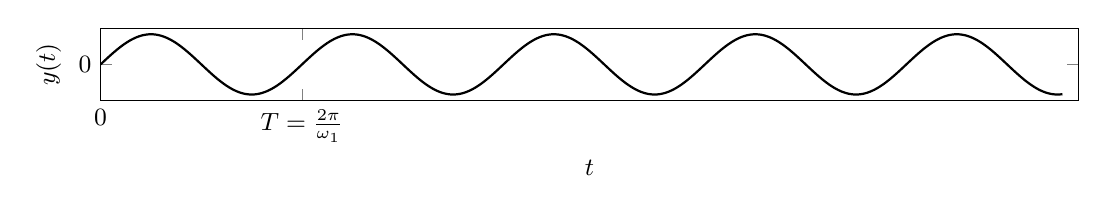
\begin{tikzpicture}
\small
\pgfmathsetmacro{\ww}{1}
\pgfmathsetmacro{\TT}{2*pi/\ww}
\begin{axis}[
width=14cm,
height=2.5cm,
xlabel={$t$},
ylabel={$y(t)$},
xmin=0.,
xmax=30.5,
ytick = {0},
xtick = {0, \TT},
xticklabels={0, $T=\frac{2\pi}{\omega_1}$},
]
\addplot+[black, thick,no marks, domain=0:30, samples=400,variable=t] { sin(deg(\ww*t)) };
\end{axis}
\end{tikzpicture}
\end{center}
Since \[y(t) = \sin(\omega_1 t) = \frac{1}{2i} \left( \mathrm{e}^{i\omega_1 t} - \mathrm{e}^{-i \omega_1 t} \right)\]
the Fourier transform of a sinusoid becomes
\[ Y(i\omega) = \frac{1}{2i} \left( 2\pi \delta(\omega_1 - \omega) - 2\pi \delta(\omega_1 + \omega) \right)\]
\end{frame}

\begin{frame}[label={sec:org3414e0c}]{Exercise 1: Fourier transform of a sinusoid}
Consider the signal below


\begin{center}
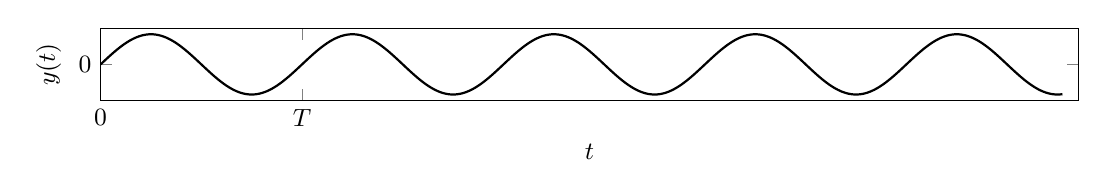
\begin{tikzpicture}
\small
\pgfmathsetmacro{\ww}{1}
\pgfmathsetmacro{\TT}{2*pi/\ww}
\begin{axis}[
width=14cm,
height=2.5cm,
xlabel={$t$},
ylabel={$y(t)$},
xmin=0.,
xmax=30.5,
ytick = {0},
xtick = {0, \TT},
xticklabels={0, $T$},
]
\addplot+[black, thick,no marks, domain=0:30, samples=400,variable=t] { sin(deg(\ww*t)) };
\end{axis}
\end{tikzpicture}
\end{center}

Which of the below is the correct Fourier transform (magnitude plot shown)?


\pgfplotsset{
dirac/.style={
mark=triangle*,
mark options={scale=0.6},
ycomb,
scatter,
visualization depends on={y/abs(y)-1 \as \sign},
scatter/@pre marker code/.code={\scope[rotate=90*\sign,yshift=-2pt]}
}
}
  \begin{tikzpicture}
  \footnotesize

  \pgfmathsetmacro{\ww}{1}
  \pgfmathsetmacro{\TT}{2*pi/\ww}
  \pgfmathsetmacro{\omegaone}{2/\TT}
  \pgfmathsetmacro{\omegatwo}{pi/\TT}
  \pgfmathsetmacro{\omegathree}{1/\TT}
  \pgfmathsetmacro{\omegafour}{2*pi/\TT}

  \begin{groupplot}[group style={group size=2 by 2, vertical sep=1.2cm, horizontal sep=1.3cm},
  width=7cm,
  height=2.5cm,
  xlabel={$\omega$ [rad/s]},
  ylabel={$|Y(i\omega)|$},
  xmin=-1.5,
  xmax=1.5,
  ytick = \empty,
  xtick = \empty,
  ]
  \nextgroupplot[xtick={-\omegaone, 0, \omegaone}, 
  xticklabels={$-\frac{2}{T}$, 0, $\frac{2}{T}$}]
  \addplot[red, thick, dirac] coordinates {(-\omegaone, 1) (\omegaone, 1)};

  \nextgroupplot[xtick={-\omegatwo, 0, \omegatwo}, 
  xticklabels={$-\frac{\pi}{T}$, 0, $\frac{\pi}{T}$}]
  \addplot[red, thick, dirac] coordinates {(-\omegatwo, 1) (\omegatwo, 1)};

  \nextgroupplot[xtick={-\omegathree, 0, \omegathree}, 
  xticklabels={$-\frac{1}{T}$, 0, $\frac{1}{T}$}]
  \addplot[red, thick, dirac] coordinates {(-\omegathree, 1) (\omegathree, 1)};

  \nextgroupplot[xtick={-\omegafour, 0, \omegafour}, 
  xticklabels={$-\frac{2\pi}{T}$, 0, $\frac{2\pi}{T}$}]
  \addplot[red, thick, dirac] coordinates {(-\omegafour, 1) (\omegafour, 1)};
  \end{groupplot}

  \node[red] at (group c1r1.center) {\huge 1};
  \node[red] at (group c2r1.center) {\huge 2};
  \node[red] at (group c1r2.center) {\huge 3};
  \node[red] at (group c2r2.center) {\huge 4};
  \end{tikzpicture}
\end{frame}
\begin{frame}[label={sec:org18f3da6}]{Exercise 2: Two sinusoids}
Consider a signal with Fourier transform  

\pgfplotsset{
dirac/.style={
mark=triangle*,
mark options={scale=0.6},
ycomb,
scatter,
visualization depends on={y/abs(y)-1 \as \sign},
scatter/@pre marker code/.code={\scope[rotate=90*\sign,yshift=-2pt]}
}}
\begin{center}
\begin{tikzpicture}
\small
\pgfmathsetmacro{\wwone}{1}
\pgfmathsetmacro{\wwtwo}{5*\wwone}
\begin{axis}[
width=14cm,
height=2.5cm,
xlabel={$\omega$ [rad/s]},
ylabel={$|Y(i\omega)|$},
xmin=-7,
xmax=7,
ymin=-0.5,
ytick=\empty,
xtick = {-\wwtwo, -\wwone, 0, \wwone, \wwtwo},
% ticklabels={$-5\omega_1$, $-\omega_1$, 0, $\omega_1$, $5\omega_1$},
]
\addplot[black, thick, dirac] coordinates {(-\wwtwo, 0.3) (-\wwone, 1) (\wwone, 1) (\wwtwo, 0.3)};
\end{axis}
\end{tikzpicture}
\end{center}

Which of the below time series could this Fourier transform correspond to?


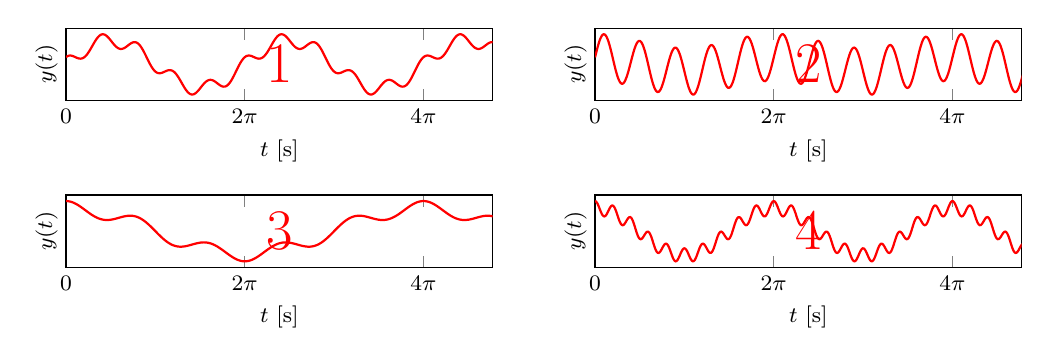
\begin{tikzpicture}
\footnotesize

\pgfmathsetmacro{\wwone}{1}
\pgfmathsetmacro{\wwtwo}{5*\wwone}

\begin{groupplot}[group style={group size=2 by 2, vertical sep=1.2cm, horizontal sep=1.3cm},
width=7cm,
height=2.5cm,
xlabel={$t$ [s]},
ylabel={$y(t)$},
xmin=0,
xmax=15,
ytick = \empty,
xtick = \empty,
domain=0:20,
samples=600,
variable=t,
]

\nextgroupplot[xtick={0, 6.28, 12.56}, xticklabels={0, $2\pi$, $4\pi$},]
 \addplot[red, thick, no marks] { sin(deg(\wwone*t)) + 0.3*cos(deg(\wwtwo*t))};

\nextgroupplot[xtick={0, 6.28, 12.56}, xticklabels={0, $2\pi$, $4\pi$},]
 \addplot[red, thick, no marks] { 0.3*cos(deg(\wwone*t)) + sin(deg(\wwtwo*t))};

\nextgroupplot[xtick={0, 6.28, 12.56}, xticklabels={0, $2\pi$, $4\pi$},]
 \addplot[red, thick, no marks] { cos(deg(0.5*\wwone*t)) + 0.3*cos(deg(0.5*\wwtwo*t))};

\nextgroupplot[xtick={0, 6.28, 12.56}, xticklabels={0, $2\pi$, $4\pi$},]
 \addplot[red, thick, no marks] { cos(deg(\wwone*t)) + 0.3*cos(deg(2*\wwtwo*t))};

\end{groupplot}

\node[red] at (group c1r1.center) {\huge 1};
\node[red] at (group c2r1.center) {\huge 2};
\node[red] at (group c1r2.center) {\huge 3};
\node[red] at (group c2r2.center) {\huge 4};
\end{tikzpicture}
\end{frame}
\begin{frame}[label={sec:org94a51df}]{Exercise 3: Fourier transform of a sampled sinusoid}
Consider the continuous and sampled signals with sampling period \(h=\frac{2}{3}T\)


 \pgfplotsset{
dirac/.style={
mark=triangle*,
mark options={scale=0.6},
ycomb,
scatter,
visualization depends on={y/abs(y)-1 \as \sign},
scatter/@pre marker code/.code={\scope[rotate=90*\sign,yshift=-2pt]}
}
}
\begin{center}
\begin{tikzpicture}
\small
\pgfmathsetmacro{\ww}{1}
\pgfmathsetmacro{\TT}{2*pi/\ww}
\pgfmathsetmacro{\TTT}{2*\TT}
\pgfmathsetmacro{\wws}{3*\ww/2}
\pgfmathsetmacro{\hh}{2*pi/\wws}
\pgfmathsetmacro{\Ttot}{60}
\pgfmathsetmacro{\Nsamples}{floor(\Ttot/\hh)}



\begin{axis}[
clip=false,
width=14cm,
height=3.5cm,
xlabel={$t$},
ylabel={$y(t)$},
xmin=0.,
xmax=\Ttot,
ytick = {0},
xtick = {0, \hh, \TT, \TTT},
xticklabels={0, $h$, $T$, $2T$},
]
\addplot+[black, thick,no marks, domain=0:\Ttot, samples=400,variable=t] { sin(deg(\ww*t)) }
       node [coordinate, pos=0.87, pin=45:{$y(t)$}] {};
\addplot+[color=blue!80!red!90, thick,dirac, domain=0:\Ttot, samples=\Nsamples+1,variable=t] { sin(deg(\ww*t))} node [coordinate, pos=0.93, pin=-45:{$y_s(t)$}] {};

\draw[blue!80!red!90, thick] (axis cs: 0,0) -- (axis cs: \Ttot, 0);

\end{axis}
\end{tikzpicture}
\end{center}

What is the frequency of the sinusoid? What is the sampling frequency \(\omega_s\) and the Nyquist frequency \(\omega_N\) in terms of the period \(T\) of the sinusoid?
\end{frame}
\begin{frame}[label={sec:orgd7314ba}]{Exercise 3: Fourier transform of a sampled sinusoid}
\small 
Consider the continuous and sampled signals with sampling period \(h=\frac{2}{3}T\)


\pgfplotsset{
dirac/.style={
mark=triangle*,
mark options={scale=0.6},
ycomb,
scatter,
visualization depends on={y/abs(y)-1 \as \sign},
scatter/@pre marker code/.code={\scope[rotate=90*\sign,yshift=-2pt]}
}
}
\begin{center}
\begin{tikzpicture}
\small
\pgfmathsetmacro{\ww}{1}
\pgfmathsetmacro{\TT}{2*pi/\ww}
\pgfmathsetmacro{\TTT}{2*\TT}
\pgfmathsetmacro{\wws}{3*\ww/2}
\pgfmathsetmacro{\hh}{2*pi/\wws}
\pgfmathsetmacro{\Ttot}{60}
\pgfmathsetmacro{\Nsamples}{floor(\Ttot/\hh)}



\begin{axis}[
clip=false,
width=14cm,
height=2.2cm,
xlabel={$t$},
ylabel={$y(t)$},
xmin=0.,
xmax=\Ttot,
ytick = {0},
xtick = {0, \hh, \TT, \TTT},
xticklabels={0, $h$, $T$, $2T$},
]
\addplot+[black, thick,no marks, domain=0:\Ttot, samples=400,variable=t] { sin(deg(\ww*t)) }
       node [coordinate, pos=0.87, pin=45:{$y(t)$}] {};
\addplot+[color=blue!80!red!90, thick,dirac, domain=0:\Ttot, samples=\Nsamples+1,variable=t] { sin(deg(\ww*t))} node [coordinate, pos=0.93, pin=-45:{$y_s(t)$}] {};

\draw[blue!80!red!90, thick] (axis cs: 0,0) -- (axis cs: \Ttot, 0);

\end{axis}
\end{tikzpicture}
\end{center}
Which of the below corresponds to the Fourier transform of the \alert{sampled signal}?

\pgfplotsset{
dirac/.style={
mark=triangle*,
mark options={scale=0.6},
ycomb,
scatter,
visualization depends on={y/abs(y)-1 \as \sign},
scatter/@pre marker code/.code={\scope[rotate=90*\sign,yshift=-2pt]}
}
}
  \begin{tikzpicture}
  \scriptsize

  \pgfmathsetmacro{\ww}{1}
  \pgfmathsetmacro{\TT}{2*pi/\ww}
  \pgfmathsetmacro{\wws}{3*\ww/2}
  \pgfmathsetmacro{\wwN}{\wws/2}

  \pgfmathsetmacro{\omegaone}{\ww-\wwN}
  \pgfmathsetmacro{\omegathree}{\wws - \ww}
  \pgfmathsetmacro{\omegafour}{\wwN/2}

  \begin{groupplot}[group style={group size=2 by 2, vertical sep=1.2cm, horizontal sep=1.3cm},
  width=8cm,
  height=2.5cm,
  xlabel={$\omega$ [rad/s]},
  ylabel={$|Y_s(i\omega)|$},
  xmin=-1.8,
  xmax=1.8,
  ymax=1.2,
  ytick = \empty,
  xtick = \empty,
  ]
  \nextgroupplot[xtick={-\wws, -\ww, -\omegaone, 0, \omegaone, \ww, \wws}, 
  xticklabels={$-\frac{3\pi}{T}$, $-\frac{2\pi}{T}$, $-\frac{\pi}{2T}$, $$,$\frac{\pi}{2T}$, $\frac{2\pi}{T}$, $\frac{3\pi}{T}$},] 
  \addplot[red, thick, dirac] coordinates {(-\ww, 1) (-\omegaone, 1) (\omegaone, 1) (\ww, 1)};
  \addplot+[black, dotted, no marks] coordinates { (-\wwN, 0) (-\wwN, 2) };
  \addplot+[black, dotted, no marks] coordinates { (\wwN, 0) (\wwN, 2) };

  \nextgroupplot[xtick={-\wws, -\ww,  0,  \ww, \wws}, 
  xticklabels={$-\frac{3\pi}{T}$, $-\frac{2\pi}{T}$,  $$, $-\frac{2\pi}{T}$, $\frac{3\pi}{T}$},] 
  \addplot[red, thick, dirac] coordinates {(-\ww, 1) (\ww, 1)};
  \addplot+[black, dotted, no marks] coordinates { (-\wwN, 0) (-\wwN, 2) };
  \addplot+[black, dotted, no marks] coordinates { (\wwN, 0) (\wwN, 2) };

  \nextgroupplot[xtick={-\wws, -\ww, -\omegathree, 0, \omegathree, \ww, \wws}, 
  xticklabels={$-\frac{3\pi}{T}$, $-\frac{2\pi}{T}$, $-\frac{\pi}{T}$, $$,$\frac{\pi}{T}$, $\frac{2\pi}{T}$, $\frac{3\pi}{T}$},] 
  \addplot[red, thick, dirac] coordinates {(-\ww, 1) (-\omegathree, 1) (\omegathree, 1) (\ww, 1)};
  \addplot+[black, dotted, no marks] coordinates { (-\wwN, 0) (-\wwN, 2) };
  \addplot+[black, dotted, no marks] coordinates { (\wwN, 0) (\wwN, 2) };

  \nextgroupplot[xtick={-\wws, -\ww, -\omegafour, 0, \omegafour, \ww, \wws}, 
  xticklabels={$-\frac{3\pi}{T}$, $-\frac{2\pi}{T}$, $-\frac{3\pi}{4T}$, $$,$\frac{3\pi}{4T}$, $\frac{2\pi}{T}$, $\frac{3\pi}{T}$},] 
  \addplot[red, thick, dirac] coordinates {(-\ww, 1) (-\omegafour, 1) (\omegafour, 1) (\ww, 1)};
  \addplot+[black, dotted, no marks] coordinates { (-\wwN, 0) (-\wwN, 2) };
  \addplot+[black, dotted, no marks] coordinates { (\wwN, 0) (\wwN, 2) };

  \end{groupplot}

  \node[red] at (group c1r1.center) {\huge 1};
  \node[red] at (group c2r1.center) {\huge 2};
  \node[red] at (group c1r2.center) {\huge 3};
  \node[red] at (group c2r2.center) {\huge 4};
  \end{tikzpicture}
\end{frame}
\begin{frame}[label={sec:orgdc41f1b}]{Alias frequency}
   To find the low frequency alias \(\omega_a<\omega_N\) of a high freqency sinusoid \(\omega_1\), The expression 
\[ \omega_a = \left| \big( (\omega_1 + \omega_N) \, \text{mod}\, \omega_s\big) - \omega_N\right|\] 
can be used.
\end{frame}

\begin{frame}[label={sec:org47ea48c}]{Aliasing example}
If a continuous-time signal with frequency content (bandwidth) \(\omega_B\) is sampled at too low sampling rate ( \(\omega_s < 2\omega_B\) ), then the energy at higher frequencies is folded onto lower frequencies. 

\begin{center}
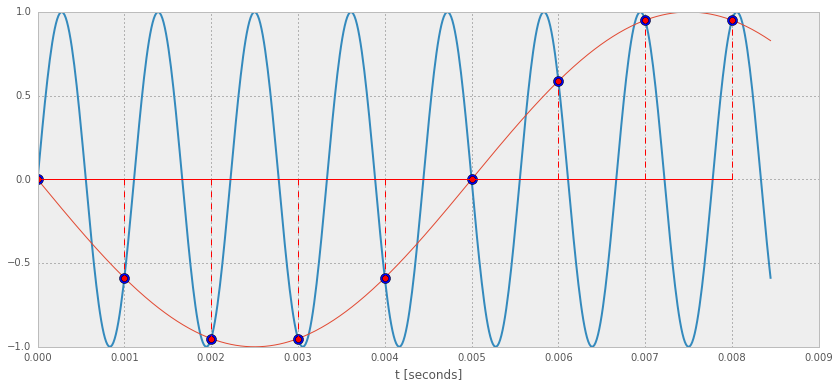
\includegraphics[width=0.6\linewidth]{../../figures/aliasing-example.png}
\end{center}
A high-frequency sinusoid ( \(\omega_1 = 1800\pi\) rad/s ) masquerading as a lower frequency sinusoid ( \(200 \pi\) rad/s ) due to aliasing when sampled with \(h=10^{-3}\) s.

\alert{Draw the spectrum (lines) of the two sinusoids. Mark the Nyquist frequency and verify that the alias frequency is obtained by folding about the Nyquist frequency.}
\end{frame}



\section{antialiasing}
\label{sec:orged21929}

\begin{frame}[label={sec:org8fc9a09}]{Noisy measurements}
\begin{columns}
\begin{column}{0.6\columnwidth}
\begin{center}
  \begin{tikzpicture}
    \node {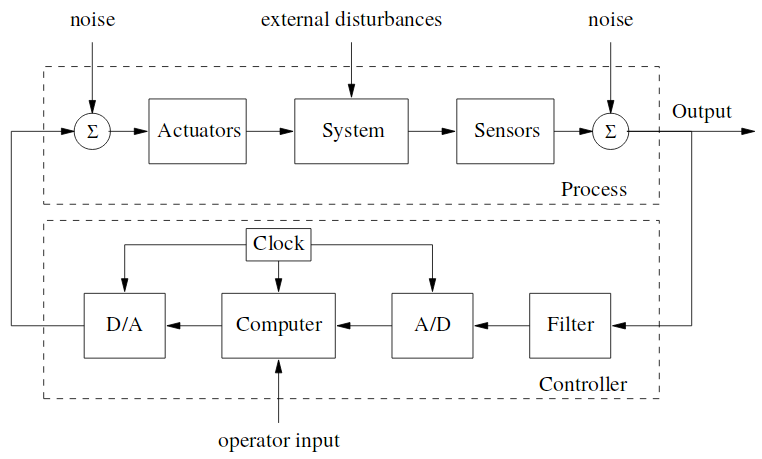
\includegraphics[width=0.99\linewidth]{../../figures/comp-contr-sys.png}};
    \node[pin=145:{60Hz mains hum}] at (2.7,2.4) {};
    \node[pin=-60:{90Hz sampling freq}] at (0.5,-1.4) {};
  \end{tikzpicture}
\end{center}
\end{column}
\begin{column}{0.4\columnwidth}
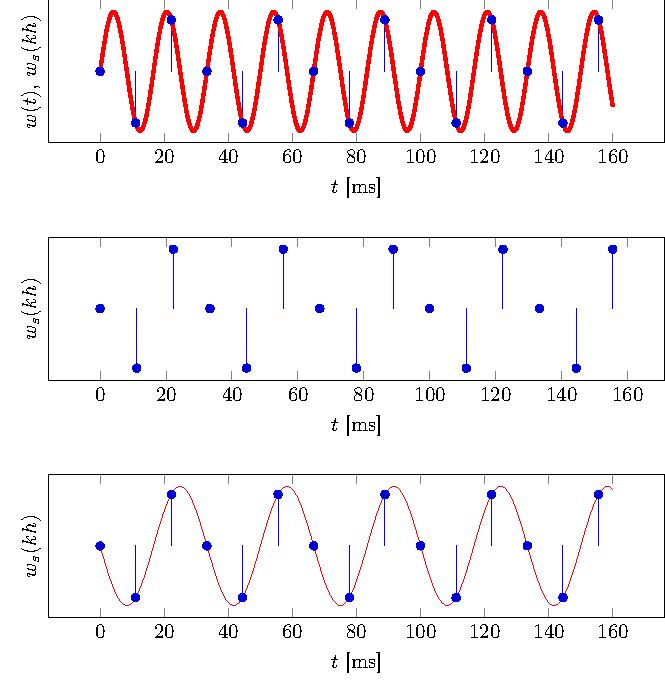
\includegraphics[width=0.99\linewidth]{../../figures/aliasing-example-60Hz}
\end{column}
\end{columns}
\end{frame}


\begin{frame}[label={sec:org68c376d}]{Antialiasing filter}
The \alert{Bessel filter} is often used. From wikipedia:
\begin{quote}
In electronics and signal processing, a Bessel filter is a type of analog linear filter with a maximally flat group/phase delay (maximally linear phase response), which preserves the wave shape of filtered signals in the passband. Bessel filters are often used in audio systems.
\end{quote}

Why use a Bessel filter as antialiasing filter?
\end{frame}


\begin{frame}[label={sec:org5a1a866}]{Antialiasing filter}
The \alert{Bessel filter} is often used. From wikipedia:
\begin{quote}
In electronics and signal processing, a Bessel filter is a type of analog linear filter with a maximally flat group/phase delay (maximally linear phase response), which preserves the wave shape of filtered signals in the passband. Bessel filters are often used in audio crossover systems.
\end{quote}

Why use as antialiasing filter?
\begin{itemize}
\item Preserves wave shapes \(\Rightarrow\) very little distortion of signals in the passband
\item Maximally linear phase response \(\Rightarrow\) \(\arg H \approx -T\omega\),  Can be modelled as a pure delay
\end{itemize}
\end{frame}
\end{document}